\section{Impulsi e segnali}\linkdest{impulse}

\begin{frame}{Signal detection}
\begin{align*}
&emf=-\TDy{t}{\Phi_{coil}}=\TDof{t}\int\,d^3r\vec{M}(\vec{r},t)\cdot\vec{\mathcal{B}}_{rec}\\
&S\propto \frac{\gamma^3B_0^2\rho_0}{T}\\
&\mathcal{B}^{rec}=\frac{\vec{B}(\vec{r}')}{I}
\end{align*}
\end{frame}

\begin{frame}[allowframebreaks]{FID, Spin echo and $T_2$ measure}
\begin{block}{Free induction decay}%
$\pi/2$ pulse lungo $x'$:
\begin{align*}
&s(t)\propto\omega_0\int d^3r \exp{-\frac{t}{T_2(r)}}B_{\perp}(\vec{r})M_{\perp}(\vec{r},0)\exp{i[(\Omega-\omega(r))t+\phi_0(\vec{r})+\theta_B(\vec{r})]}\\
&\phi(\vec{r},t)=-\omega(r)t+\phi_0(\vec{r})=-\gamma B_z(\vec{r})t+\phi_0(\vec{r})
\end{align*}
Possibilit\'a che lòa frequenza di precessione cambi con la posizione $\omega(\vec{r})$
%B_x=B_{\perp}\cos{\theta_b}
\end{block}
\begin{block}{Repeated FID}
\begin{figure}[!ht]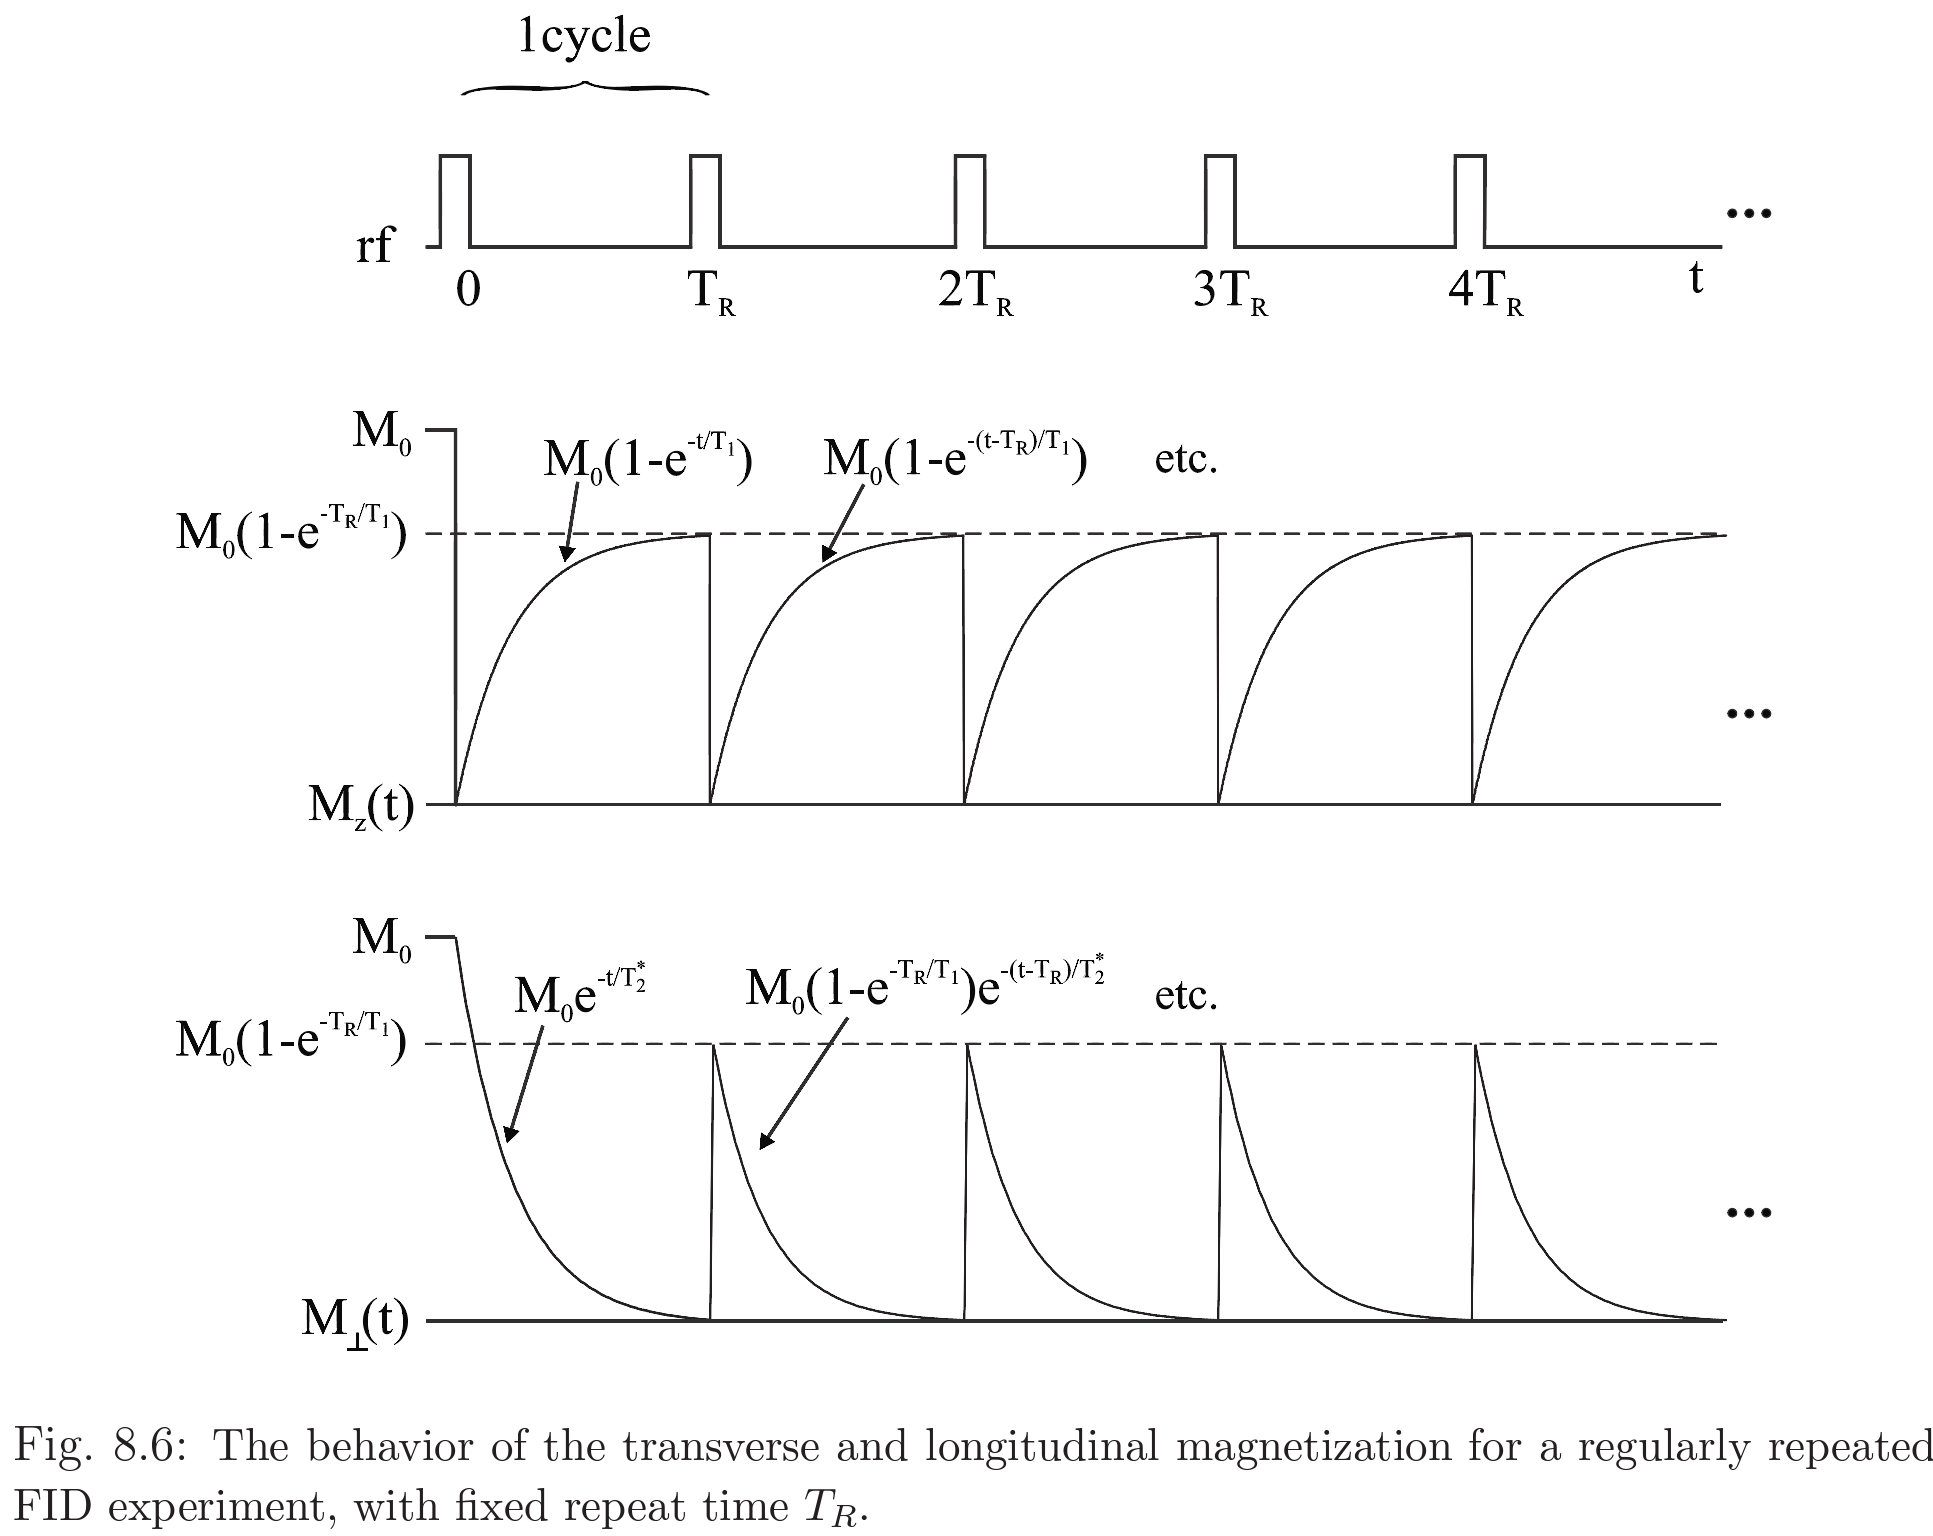
\includegraphics[trim={0cm 0cm 0 0},clip, keepaspectratio,width=0.4\textwidth]{FIDrep}\label{fig:FIDrep}\end{figure}
\end{block}
\end{frame}

\begin{frame}{$T_2*$ decay: dephasing of magnetization.}
%succo
\begin{align*}
&\frac{1}{T_2*}=\frac{1}{T_2}+\frac{1}{T_2'}\\
&M_+(\vec{r},t)=M_+(\vec{r},0)\exp{-\frac{t}{T_2*}}\\
&\phi(\vec{r},t)=-\gamma[B_0+\Delta B(\vec{r})]t
\end{align*}
$T_2'$ is machine/sample dependent $B_0$ inhomogeneities and is recoverable, $T_2$ is thermodynamic relaxing: $\sum_{sample}\exp{i\phi(\vec{r},t)}\to0$. Often $T_2'\ll T_2$.

\begin{block}{$T_2$ measure. Spin-echo.}
Impulso $(\pi/2)_{x'}$ determina spin (excess) lungo $y'$. $\Delta B(\vec{r})\neq0$ implica dephasing:
\begin{equation*}
\phi(\vec{r},t)=-\gamma\Delta B(\vec{r})t\quad 0\leq t\leq\tau
\end{equation*}
Applico impulso di $\pi$ attorno a $y'$:
\begin{align*}
&\phi(\vec{r},\tau+)=-\phi(\vec{r},\tau-)=\gamma\Delta B(\vec{r})\tau\\
&\phi(\vec{r},t)=-\phi(\vec{r},\tau)-\gamma\Delta B(\vec{r})(t-\tau)=-\gamma\Delta B(\vec{r})(t-t_E)
\end{align*}
\end{block}
\begin{block}{Misura $T_2$.}
%succo
\begin{align*}
&s(T_E)\propto\omega_0\exp{-\frac{T_E}{T_2}}\int d^3 rB_{\perp}M_{\perp}(\vec{r},0)\\
&T_2=\frac{T_E'-T_E}{\ln{[s(T_E)/s(T_E')]}}
\end{align*}
\end{block}
\end{frame}

\begin{wordonframe}{Spin-ECHO}
\begin{block}{Spin-echo exponential}
\begin{align*}
&(\TDy{t}{(M_+)})'=-R_2^{se}M_+\\
&R_2^{se}=\begin{pmatrix}R_2'+R_2\\-R_2'+R_2\\R_2'+R_2\end{pmatrix}\\
&M_{\perp}(t)=M_{\perp}(t_0)\exp{-(t-t_0)R_2^{se}}\\
&=M_{\perp}(0)\begin{pmatrix}\exp{-\frac{r}{T_2*}}\ 0<t<\tau\\\exp{-\frac{t}{T_2}}\exp{-\frac{(T_E-t)}{T_2'}}\ \tau<t<2\tau=T_E\\ \exp{-\frac{t}{T_2}}\exp{-\frac{(t-T_E)}{T_2'}}=\exp{-\frac{t}{T_2*}}\exp{-\frac{T_E}{T_2'}} \end{pmatrix}
\end{align*}
$T_2$ intrinsic rapid time fluctuation of local field.
\end{block}
Misure con $T_R\leq T_1$: ottimizzazione.
\end{wordonframe}

\begin{frame}[allowframebreaks]{Inversion recovery and $T_1$ measure - Spin-echo inversion recovery.}
Impulso $\pi$ attorno $x'$ e a $T_I$ di $\pi/2$
\begin{align*}
&M_z(0+)=-M_0\\
&M_z(t)=-M_0\exp{-\frac{t}{T_1}}+M_0(1-\exp{-\frac{t}{T_1}})\ 0<t<T_I\\
&\magort{}(t)=|M_0(1-2\exp{-\frac{T_I}{T_1}})|\exp{-\frac{(t-T_I)}{T_2*}}\\
&T_I^{null}=T_1\ln{2}
\end{align*}

\begin{figure}[!ht]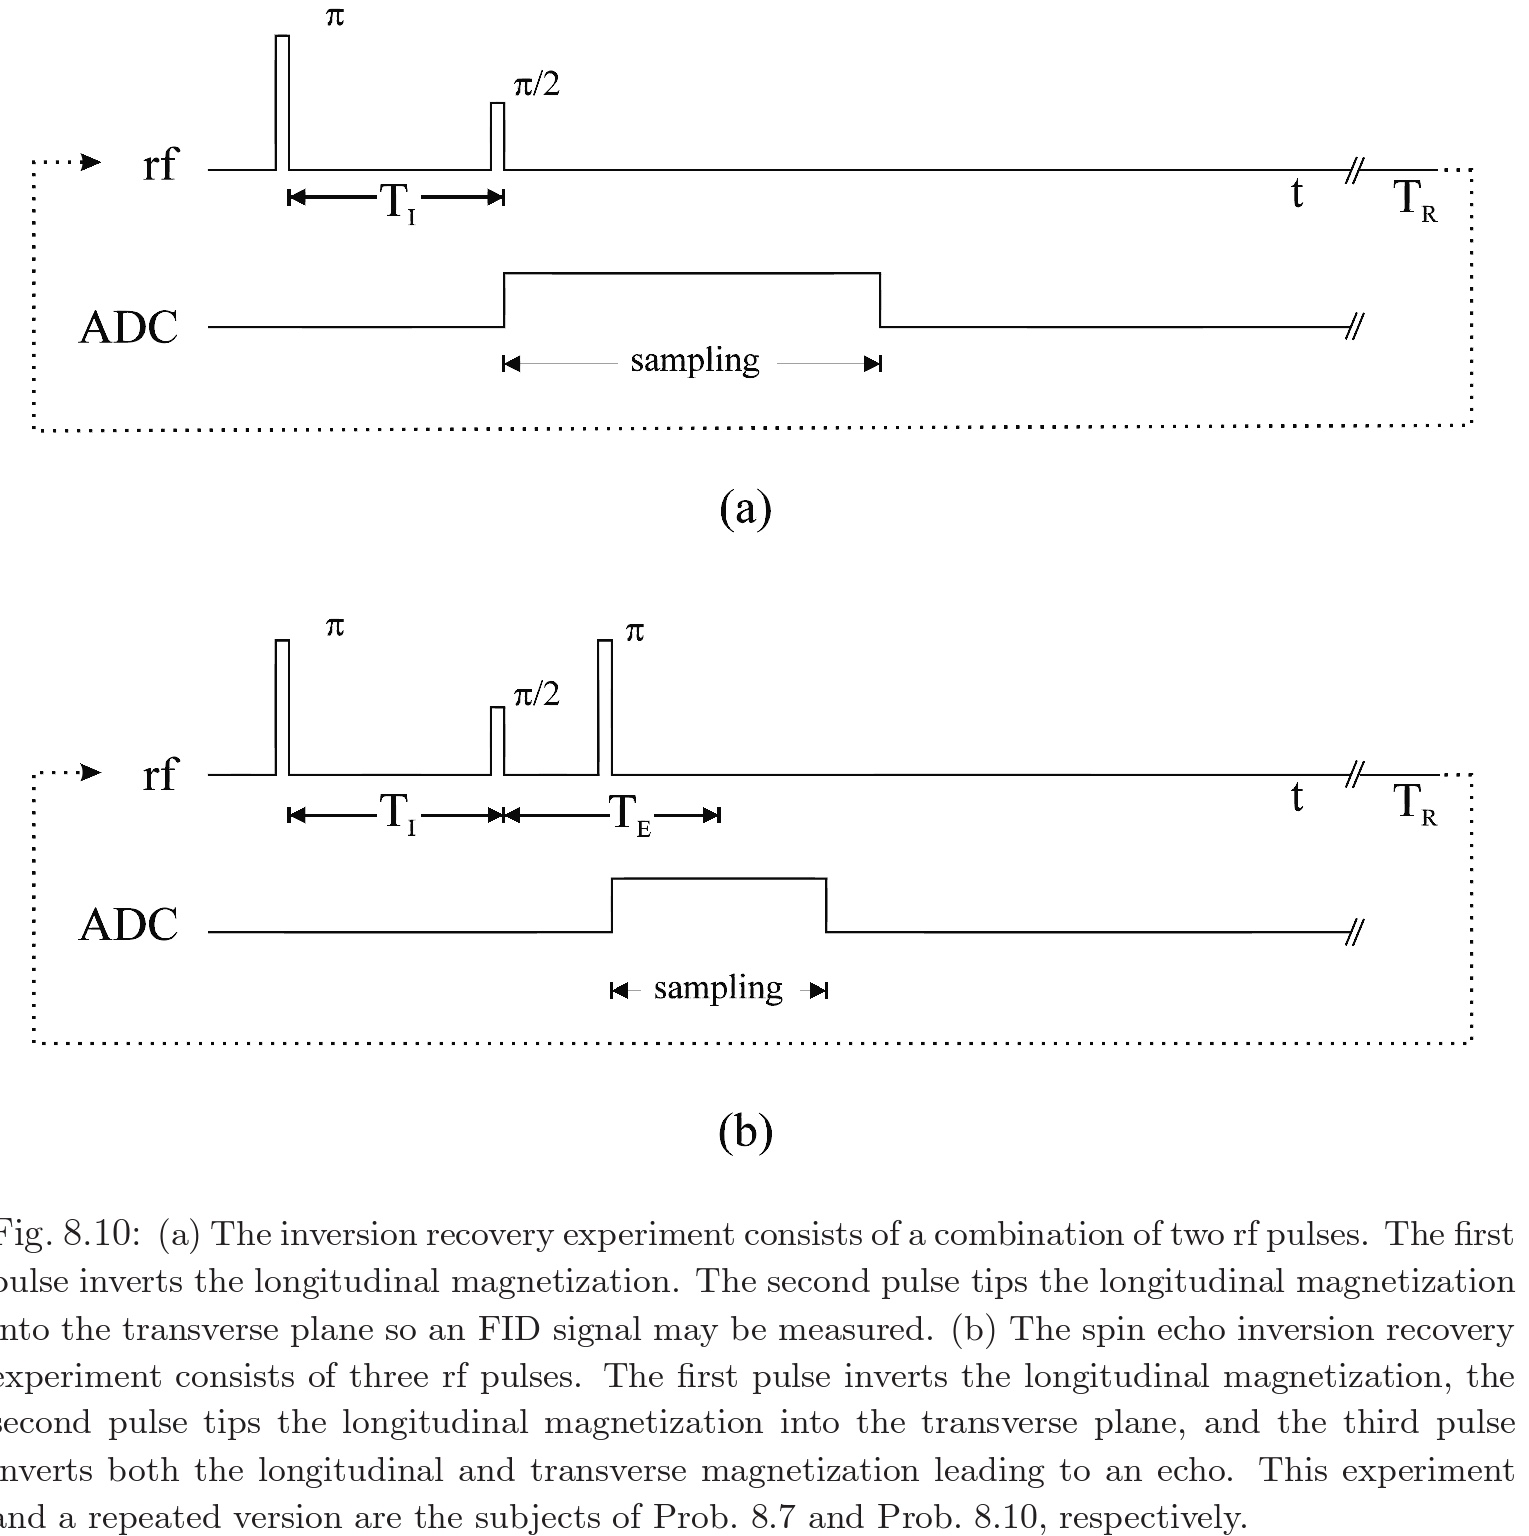
\includegraphics[trim={0cm 0 0 0},clip, width=0.9\textwidth]{IR-SE-sampling}
\label{fig:IR-SE-sampling}\end{figure} 
\begin{figure}[!ht]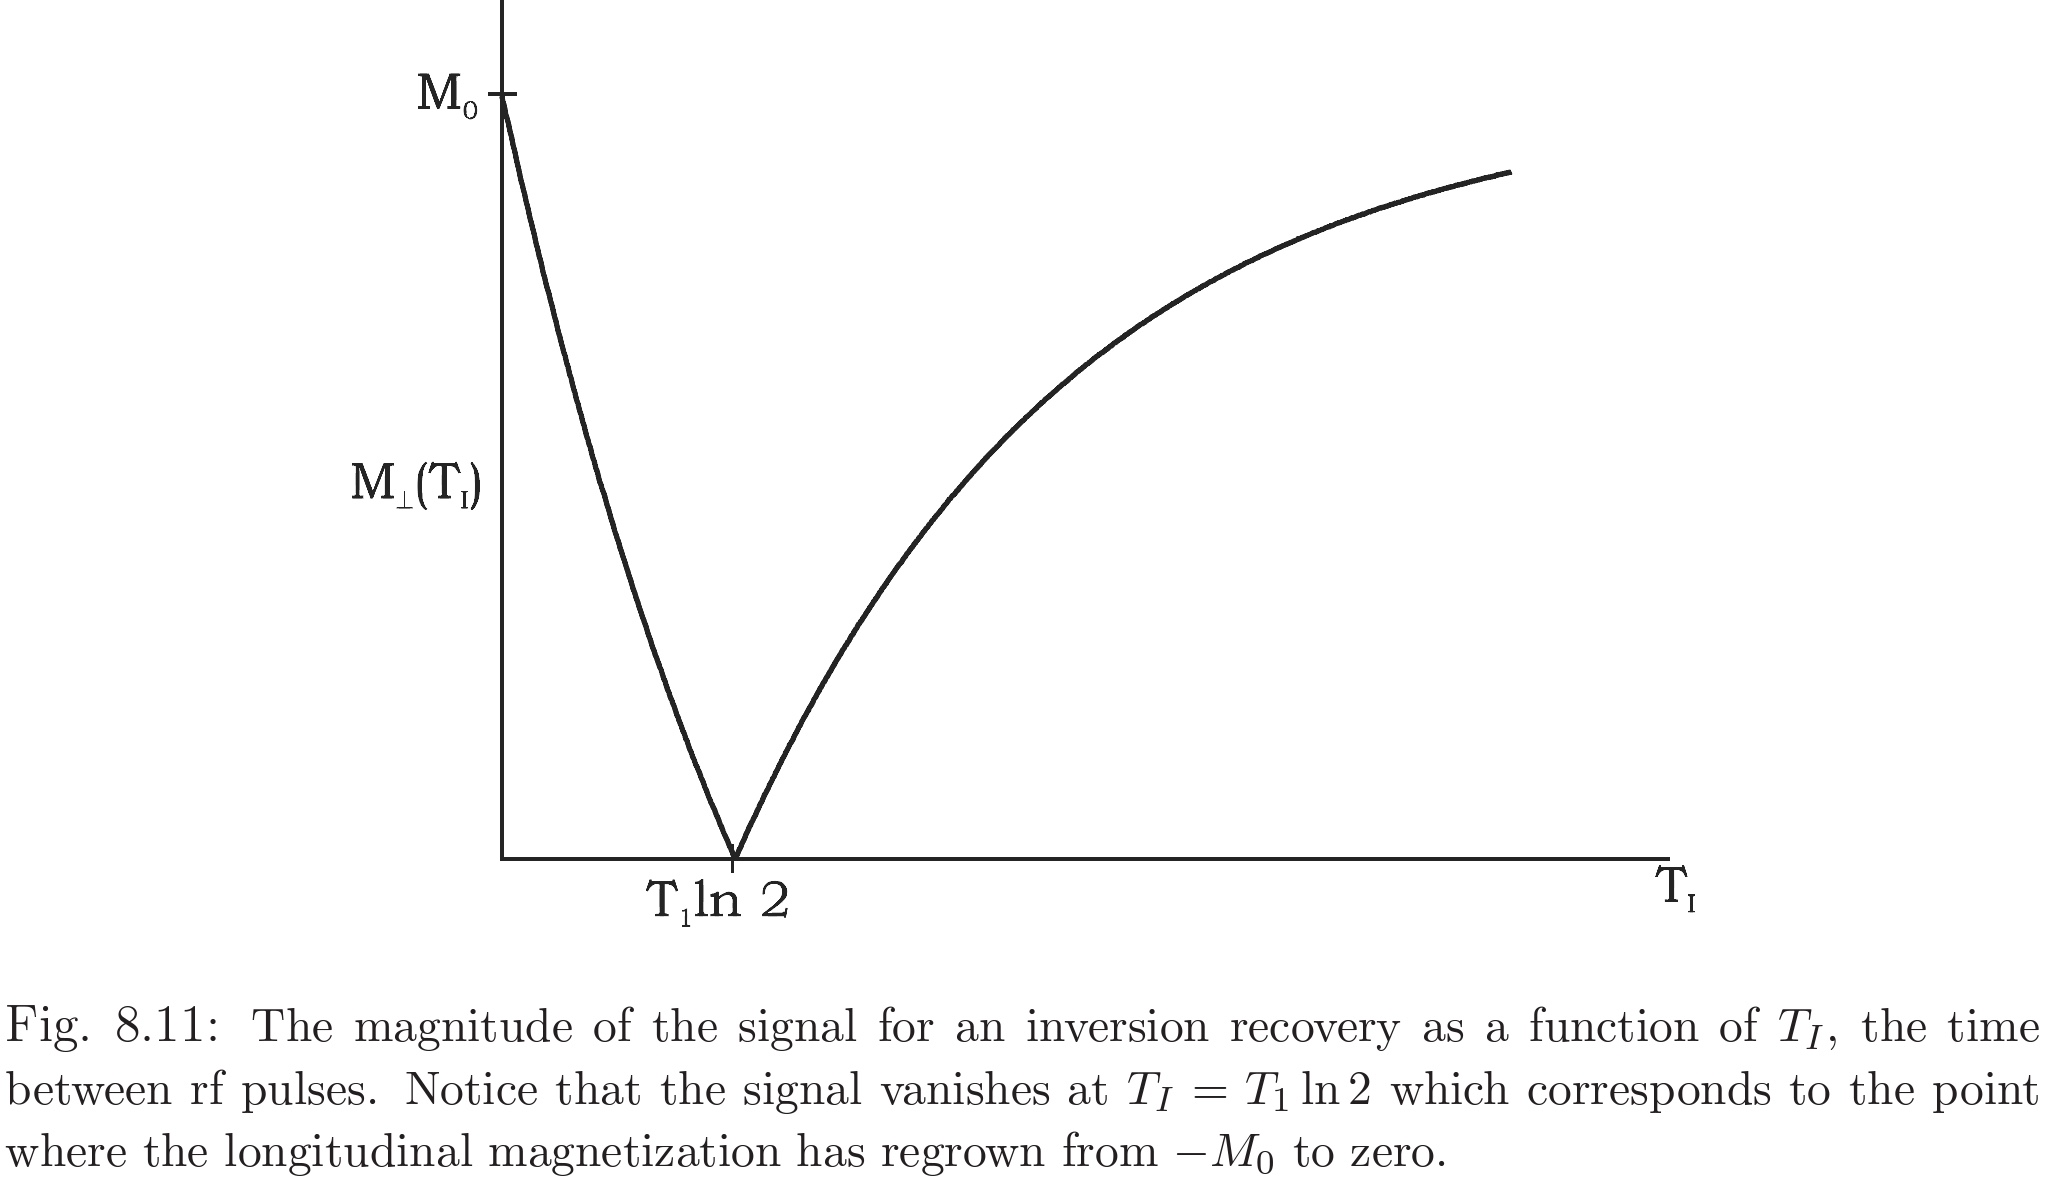
\includegraphics[trim={0cm 0 0 0},clip,width=0.9\textwidth]{IRvsTI}
\label{fig:IRvsTI}
\end{figure}

\end{frame}

\begin{frame}{Chemical shift and NMR spectroscopy}
%succo
Broadband RF excitation: complicated FID signal
\begin{align*}
&\omega_{0i}=\gamma_iB_0
\end{align*}
Determinazioni specie nucleari nel campione (excited by pulse spectrum).
Shielding constant: linear response of electrons to $B_{ext}$:
\begin{align*}
&B_{shift}(j)=(1-\sigma_j)B_0\to f_{\sigma}=-\sigma\gammabar B_0\\
&s(t)=\sum_jN_j\exp{i\gamma\sigma_jB_0t}
\end{align*}
\end{frame}

\section{Imaging: phase encoding, k-spazio, imaging equation}\linkdest{imaging}

\begin{frame}[allowframebreaks]{Fourier imaging, gradient echo and K-space}
Rilassamento dopo $\pi/2$-pulse:$M_{\perp}=M_0(\vec{r})$.
\begin{block}{Aggiungo campo che varia linearmente lungo z}
%succo
\begin{align*}
&s(t)\propto\int d^3 r\rho(\vec{r})\exp{i[\Omega t+\phi(\vec{r},t)]}\\
&B_z(z,t)=B_0+zG(t)\ \Rightarrow\ \omega=\omega_0+\omega_G(z,t)
\end{align*}
Frequency encoding: $\omega_G=\gamma zG(t)$.
\begin{equation*}
\phi_G(z,t)=-\int_0^td t'\omega_G(z,t')=-\gamma z\int_0^td t'G(t)
\end{equation*}
\end{block}
\begin{block}{1D imaging equation}
%succo
\begin{equation*}
s(t)=\int d z\rho(z)\exp{i\phi_G(z,t)}
\end{equation*}
$\rho$ effective spin density
\end{block}
\begin{figure}[!ht]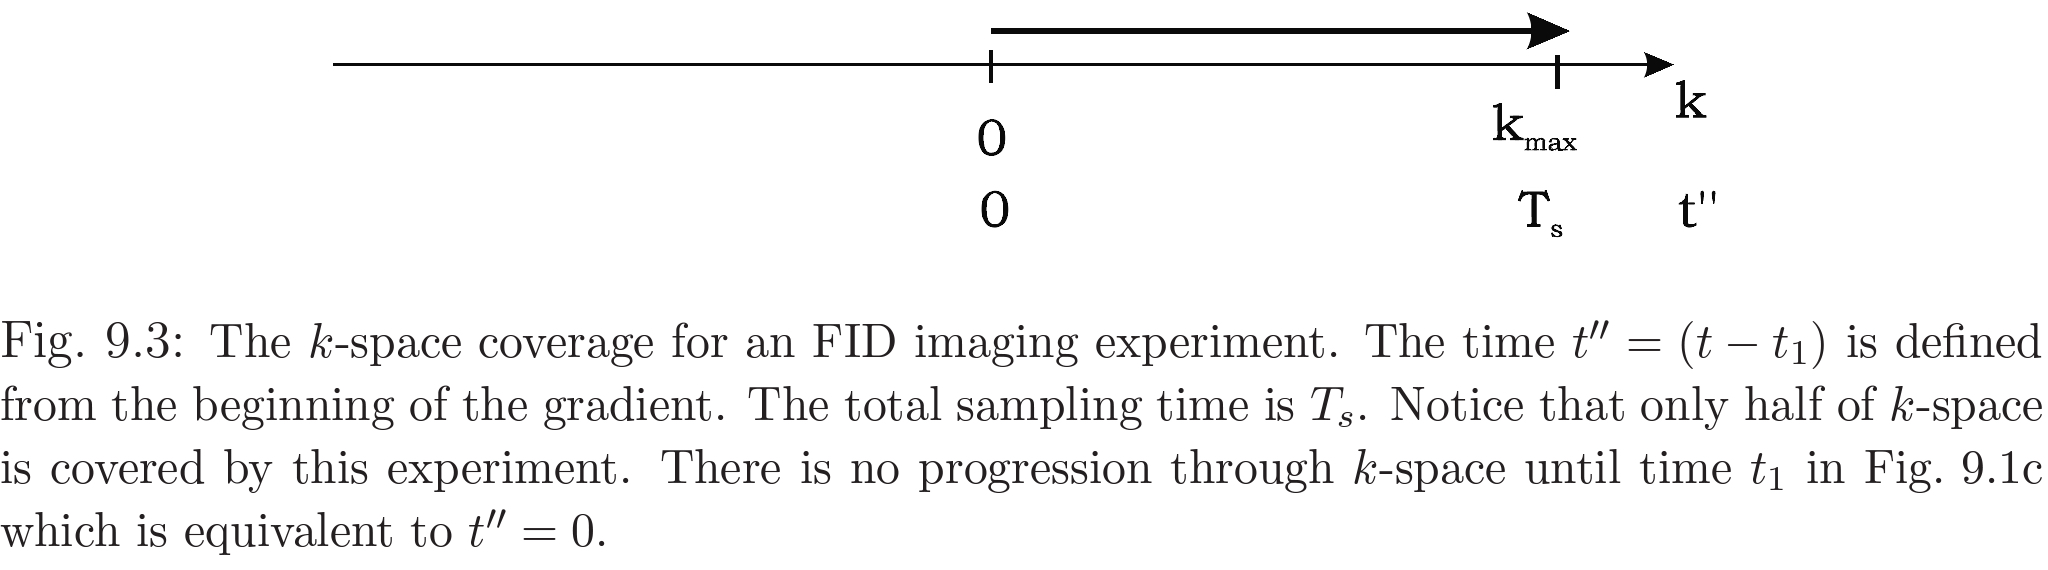
\includegraphics[trim={0cm 0cm 0 0},clip, keepaspectratio,width=\textwidth]{FID-k}\label{fig:FID-k}\end{figure}
\end{frame}

\begin{wordonframe}{Effective spin density}
\begin{align*}
M_0=\frac{1}{4}\rho_0(\vec{r})\frac{\gamma^2\hbar^2}{KT}\\
\rho(\vec{r})=\omega_0\Lambda B_{\perp}M_0
\end{align*}
\end{wordonframe} 

\begin{frame}{K-spazio}
\begin{align*}
s(k)=\int d z\rho(z)\exp{-i2\pi kz}
\end{align*}
Per gradiente uniforma lungo z $s(k)$ \'e la trasformata di Fourier della "densit\'a effettiva di spin del campione.
\begin{block}{Antitrasformata del segnale \'e la densit\'a spaziale}
\begin{equation*}
\rho(z)=\int d ks(k)\exp{i2\pi kz}
\end{equation*}
\end{block}
\begin{block}{Coverage of K-space}
Campionamento uniforme: sampling at constant rate in presence of constant gradient.
\begin{equation*}
k=\gammabar\int_0^tG(t')d t'
\end{equation*}
\end{block} 
\end{frame}

\begin{frame}{two spin system}
Two spin at $z=\pm z_0$: in rotating frame they preceed clock/anticlock-wise.
\begin{align*}
&\phi(\pm z_0,t)=\mp\gamma Gz_0(t-t_1)\\
&s(t)=s_0[\exp{-i\gamma Gz_0t}+\exp{i\gamma Gz_0t}]\\
&=2s_0\cos{(\gamma G t z_0)}=2s_0\cos{(2\pi kz_0)}\\
&0\leq t\leq t_2:\ 0\leq k\leq k_2=\gammabar Gt_2
\rho(z)=\intsinf{}d k2s_0\cos{(2pi kz_0)}\exp{i2\pi kz}\\
&=s_0[\delta(z+z_0)+\delta(z-z_0)]
\end{align*}

\end{frame}

\begin{frame}{Gradient echo}
%succo
\begin{figure}[!ht]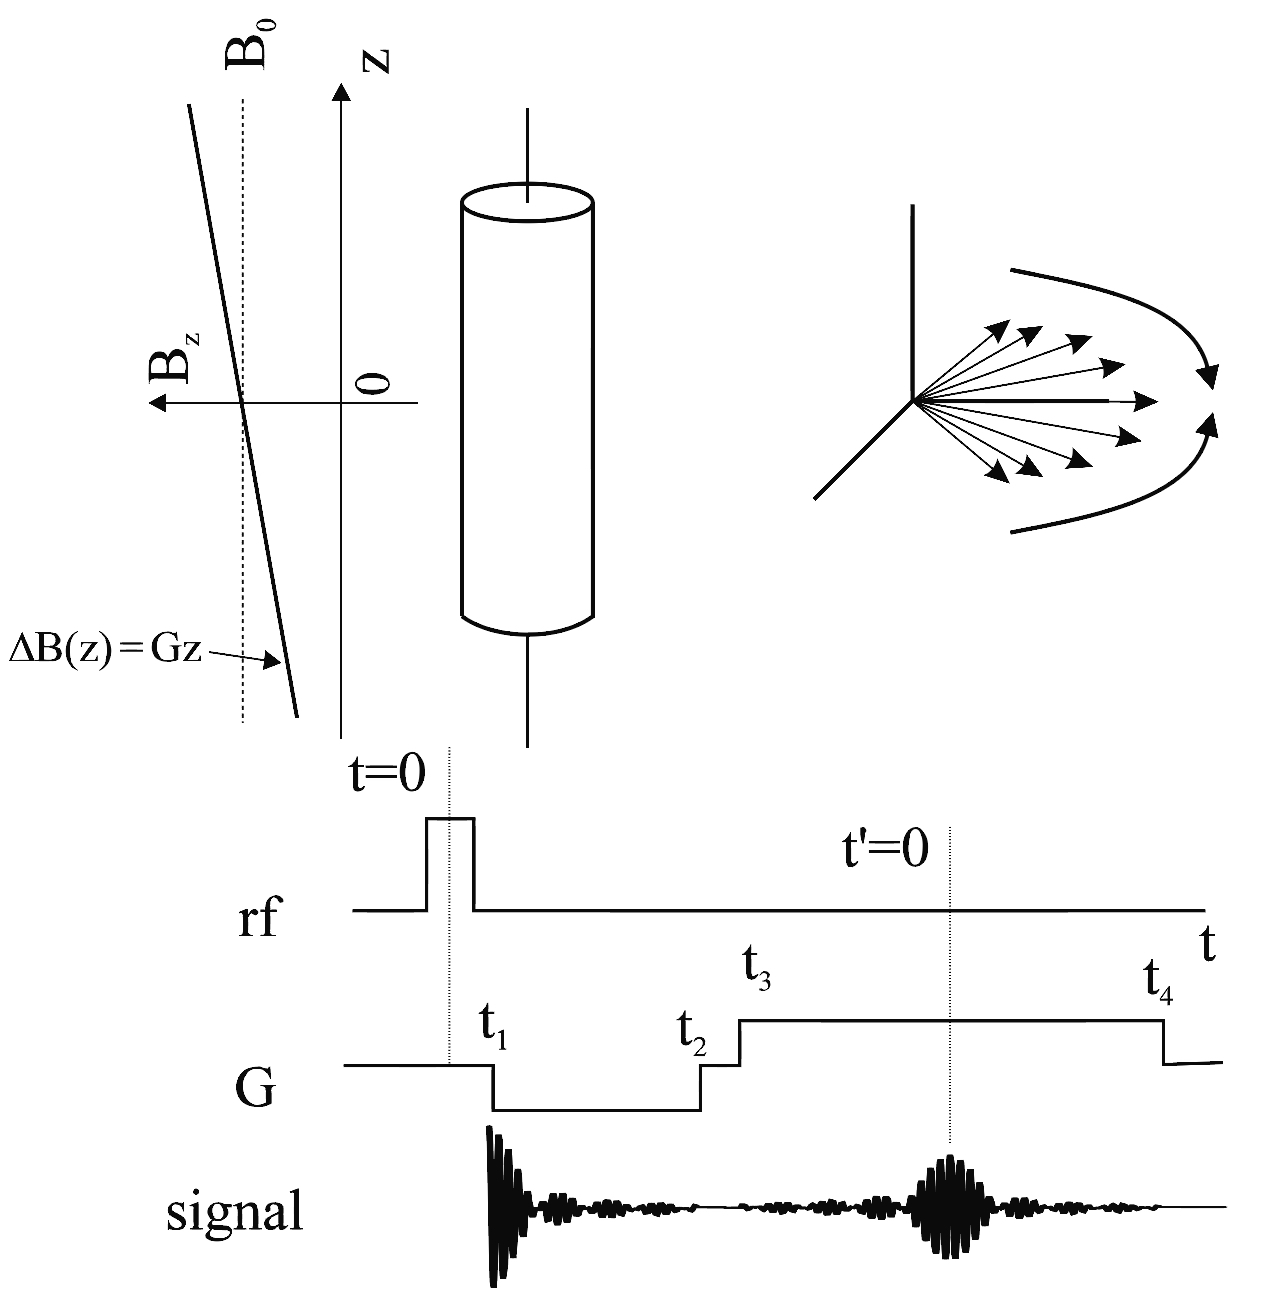
\includegraphics[trim={0cm 0cm 0 0},clip, keepaspectratio,height=0.9\textheight]{GEimaging}\end{figure}

\end{frame}

\begin{wordonframe}{Gradient echo}
\begin{align*}
&s(t')=\int d z\rho(z)\exp{-i\gamma Gzt'}:\ -\frac{t_4-t_3}{2}\leq t'\leq \frac{t_4-t_3}{2}
\end{align*}
\end{wordonframe}

\begin{frame}[allowframebreaks]{Spin-echo imaging}
%succo
\begin{figure}[!ht]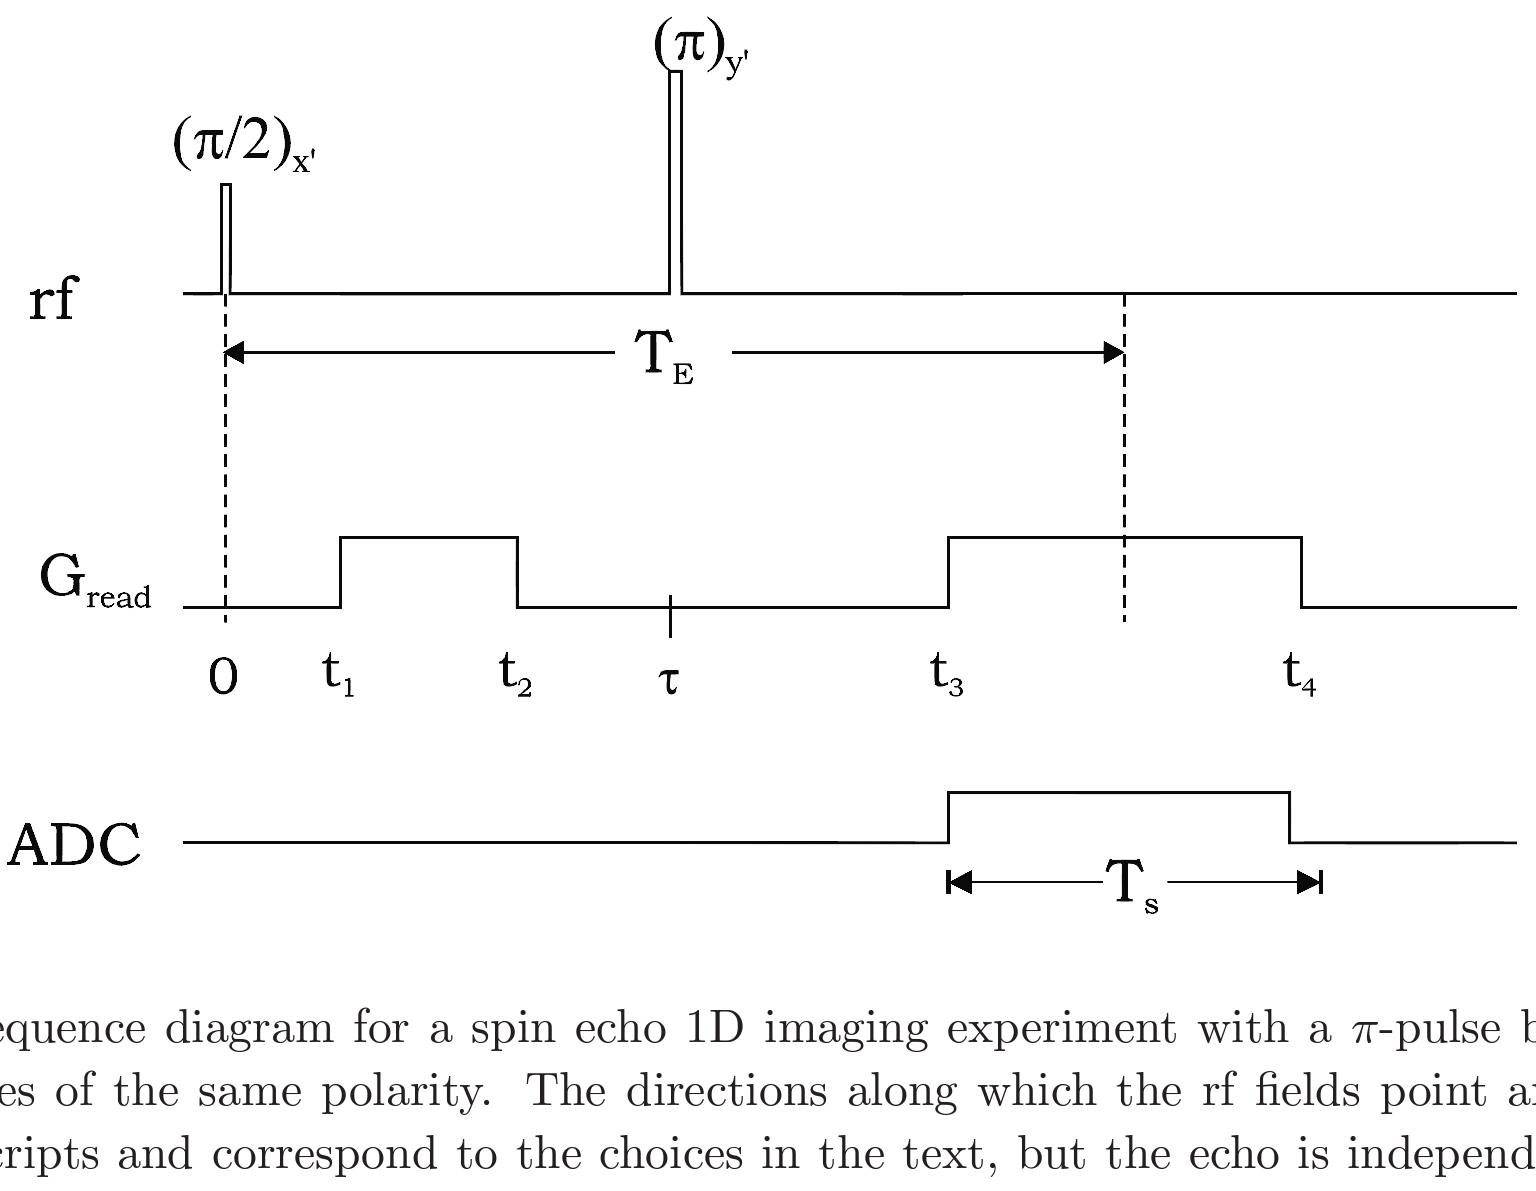
\includegraphics[trim={0cm 0cm 0 0},clip, keepaspectratio,height=0.45\textheight]{SEimaging}\end{figure}
\begin{figure}[!ht]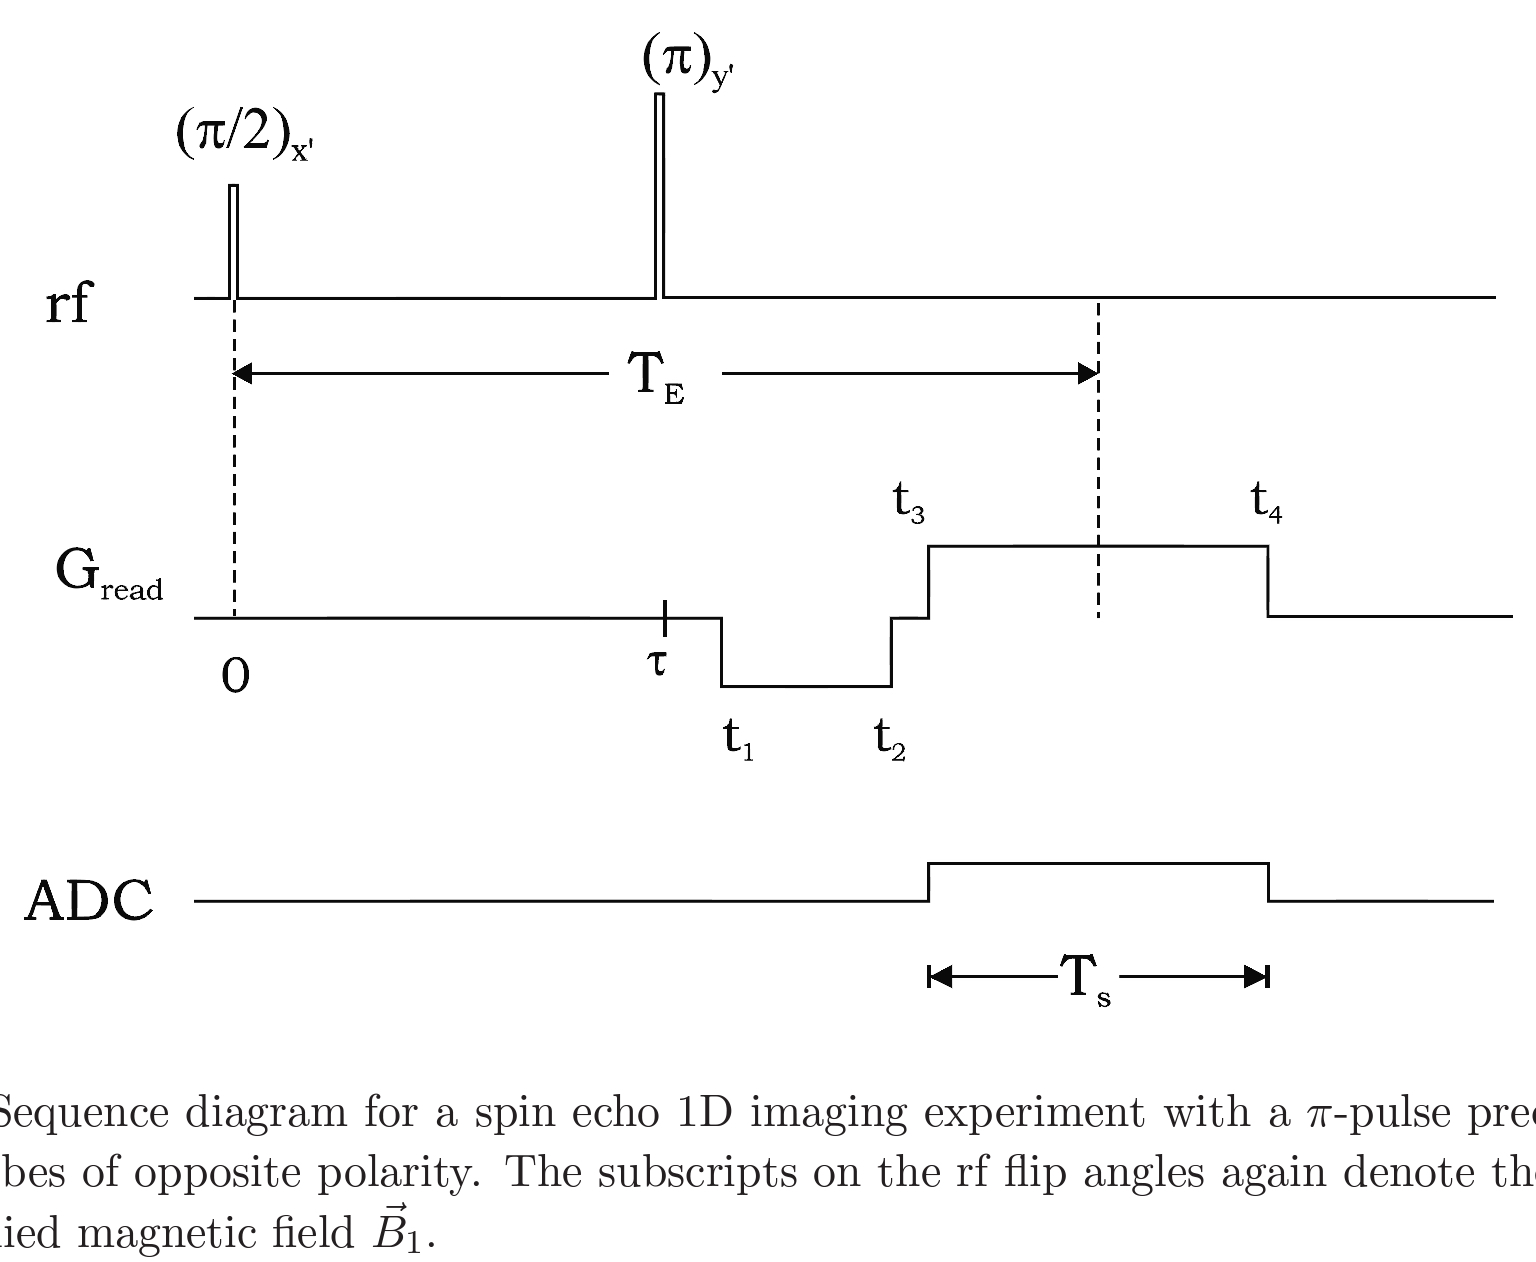
\includegraphics[trim={0cm 0cm 0 0},clip, keepaspectratio,height=0.45\textheight]{SEtotimaging}\end{figure}
\end{frame}

\begin{wordonframe}{Spin echo imaging}
Gradient echo refocus phase induced by gradient but does NOT refocus dephasing due static field inhomogeneities.

\begin{align*}
&\phi(z,t)=-\gamma\Delta B(z)t-\gamma Gz(t-t_1):\ t_1<t<t_2\\
&(\pi)_{y'},\ t=\tau:\ \phi\to-\phi\\
&\phi(z,t)=\gamma\Delta B(z)\tau+\gamma Gz(t_2-t_1)-\gamma\Delta B(z)(t-\tau)\\
&-\gamma Gz(t-t_3):\ t_3<t<t_4
\end{align*}
Total phase induced by $B_0/G$ inhomogeneities has been refocused.
Si ha:
\begin{align*}
&\phi(z,T_E)=0:\ 2\tau=t_3+(t_2-t_1)
\end{align*}
\end{wordonframe}


\begin{frame}{K-space coverage}
\begin{figure}[!ht]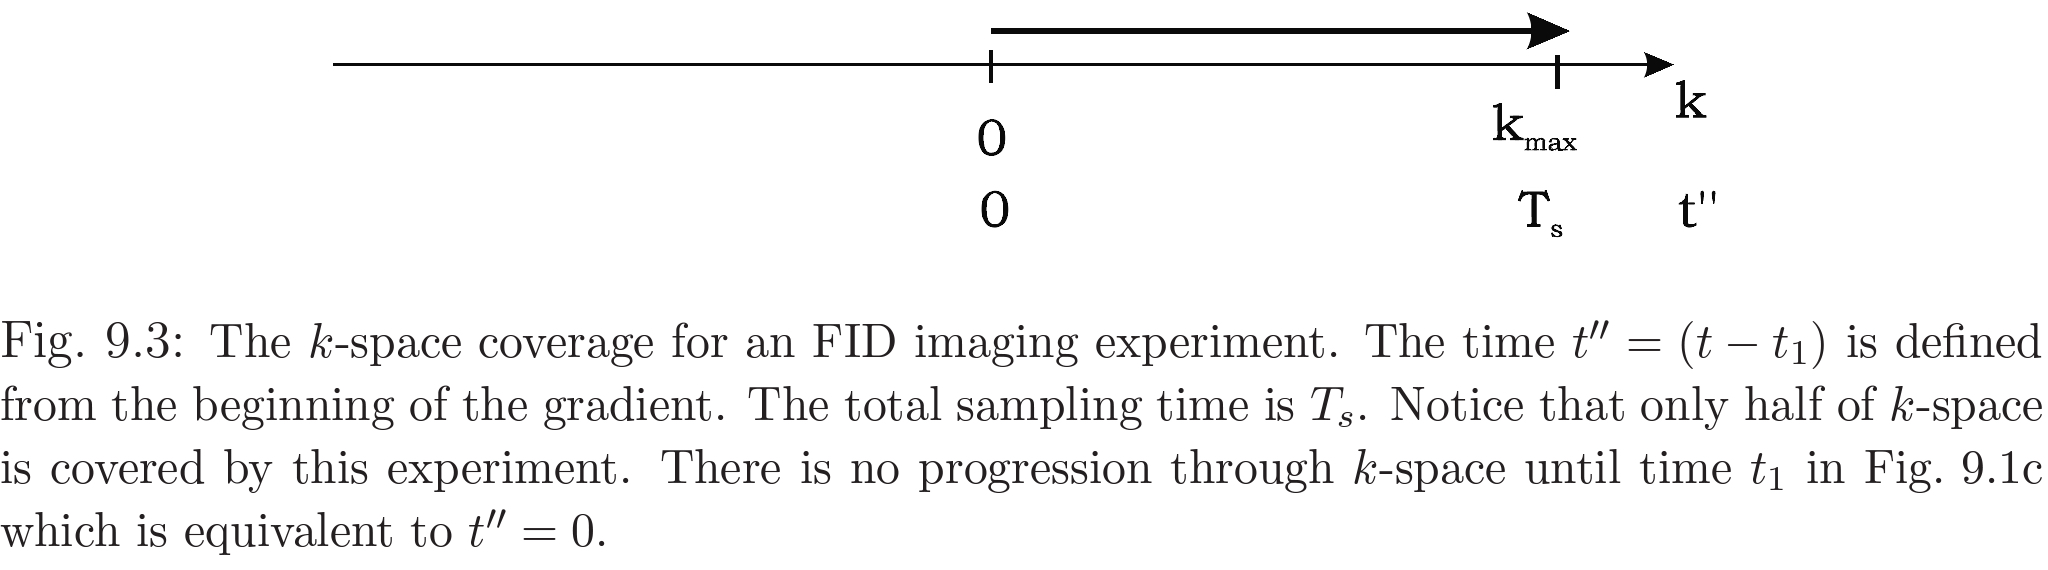
\includegraphics[trim={0cm 5cm 0 0},clip, keepaspectratio,height=0.3\textheight]{FID-k}\end{figure}

\begin{figure}[!ht]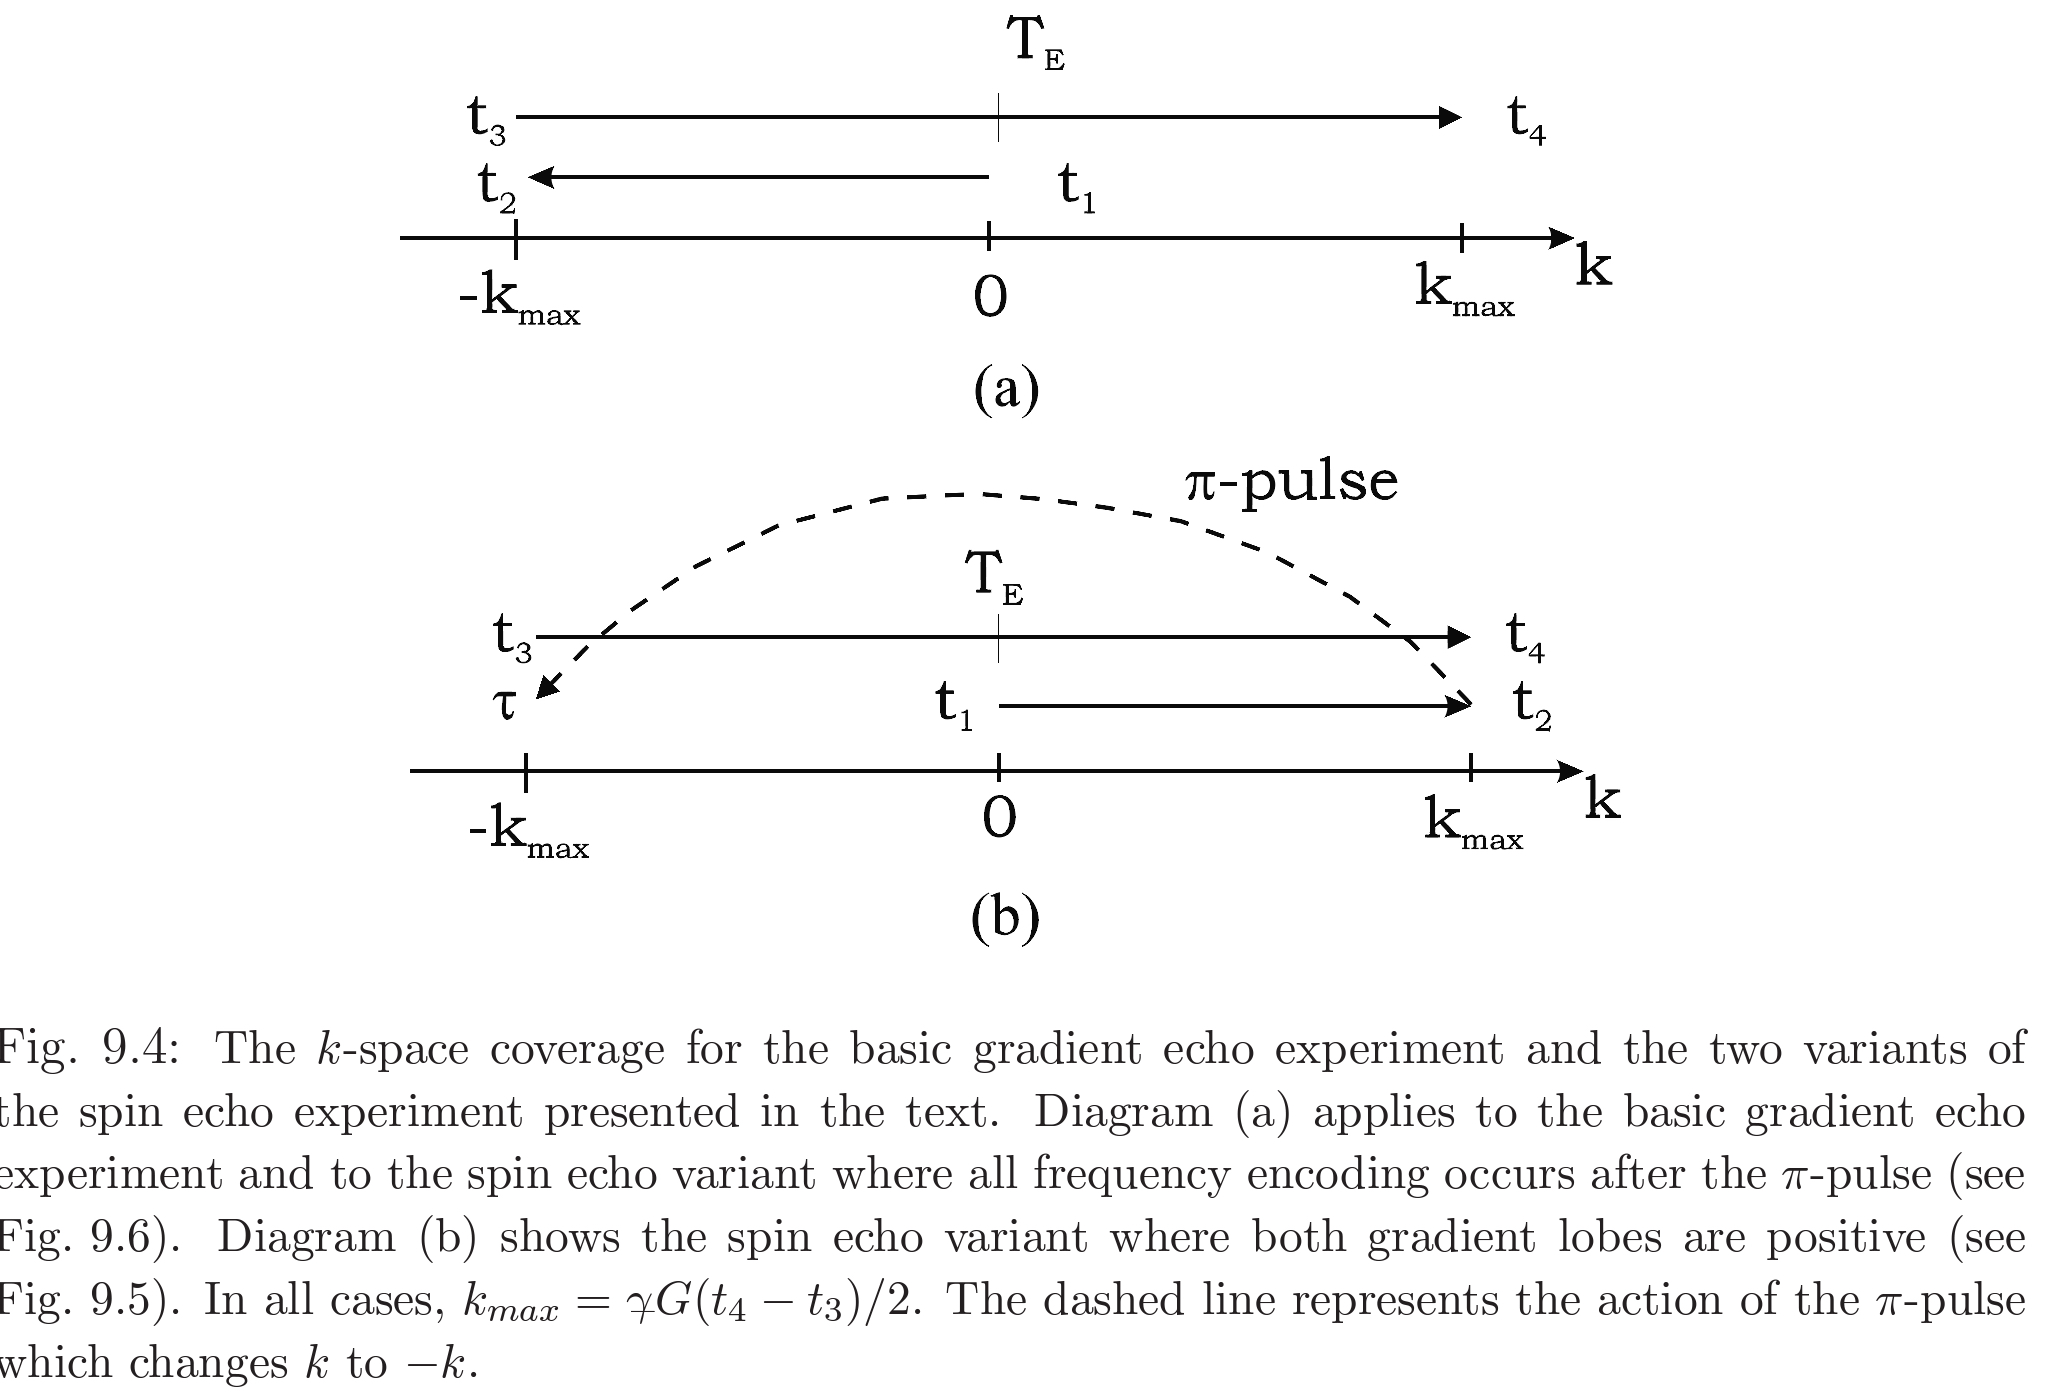
\includegraphics[trim={0cm 0cm 0 0},clip, keepaspectratio,height=0.45\textheight]{SE-GE-k}\end{figure}
\end{frame}

\begin{frame}{3D imaging}
\begin{columns}[T]
\begin{column}{0.5\textwidth}
\begin{figure}[!ht]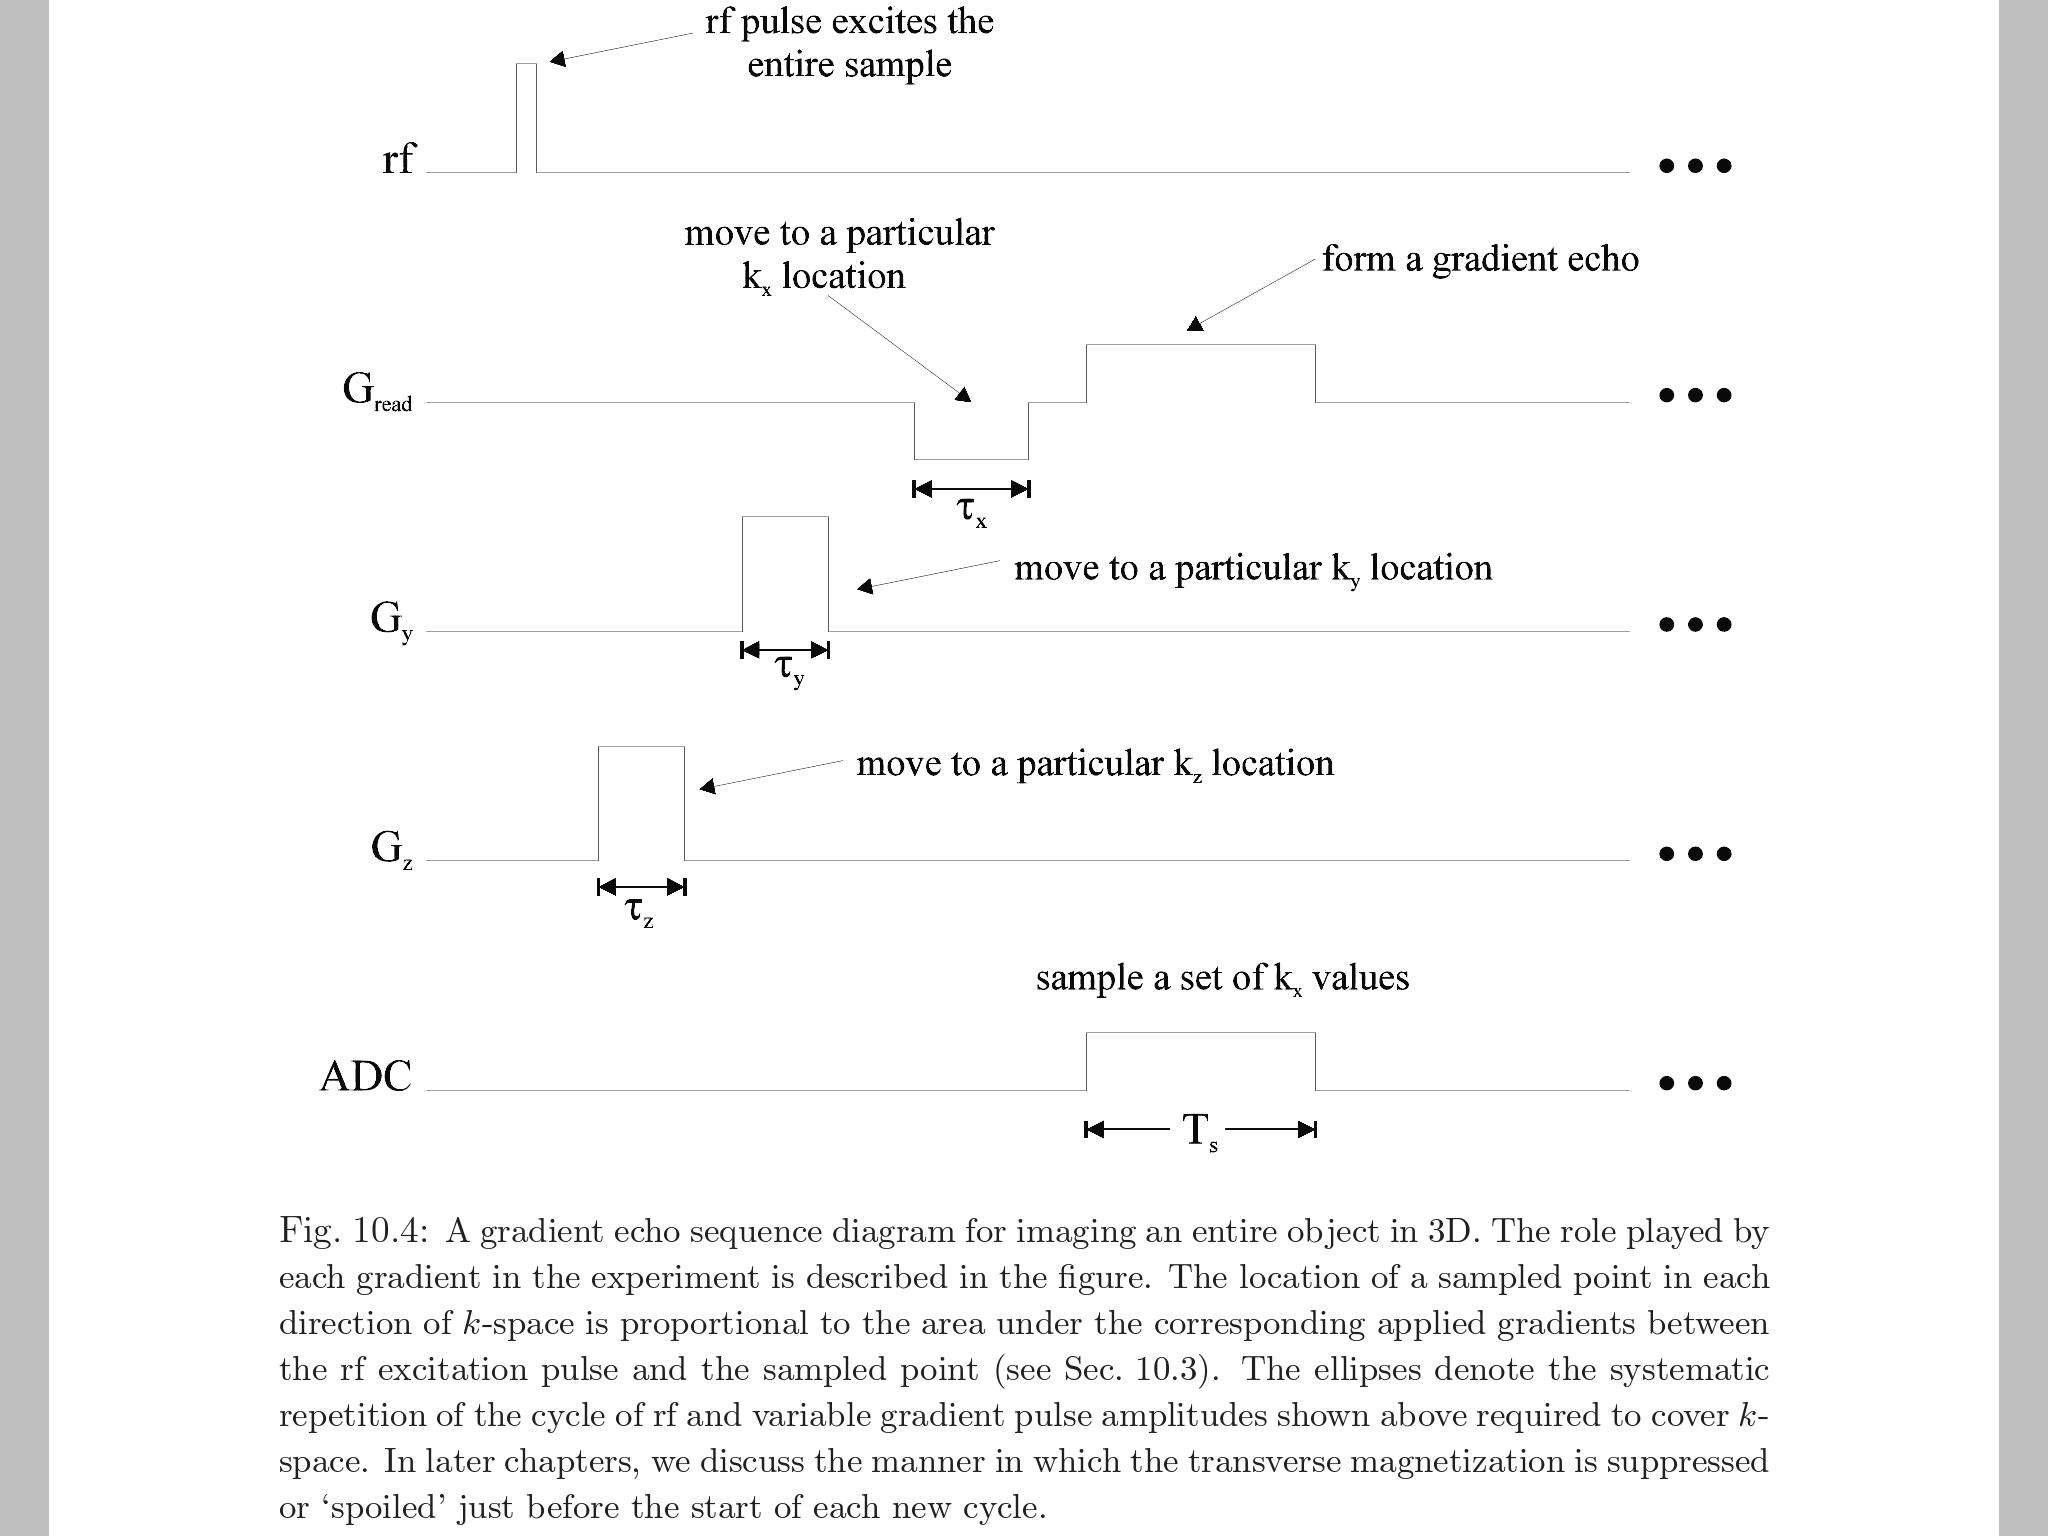
\includegraphics[trim={0cm 0cm 0 0},clip, keepaspectratio,width=0.99\textwidth]{3Dimaging}\label{fig:3Dimaging}\end{figure}
\end{column}
\begin{column}{0.5\textwidth}
\begin{align*}
&s(\vec{k})=\int d^3 r\rho(\vec{r})\exp{-i2\pi \scap{k}{r}}\\
&k_i(t)=\gammabar\int_0^tG_i(t')d t'\\
&\mathcal{F}s(\vec{k})\propto\rho(\vec{r})
\end{align*}
\end{column}
\end{columns}
\end{frame}

\begin{frame}{2D multi-slice imaging}
\begin{columns}[T]
\begin{column}{0.55\textwidth}
\begin{figure}[!ht]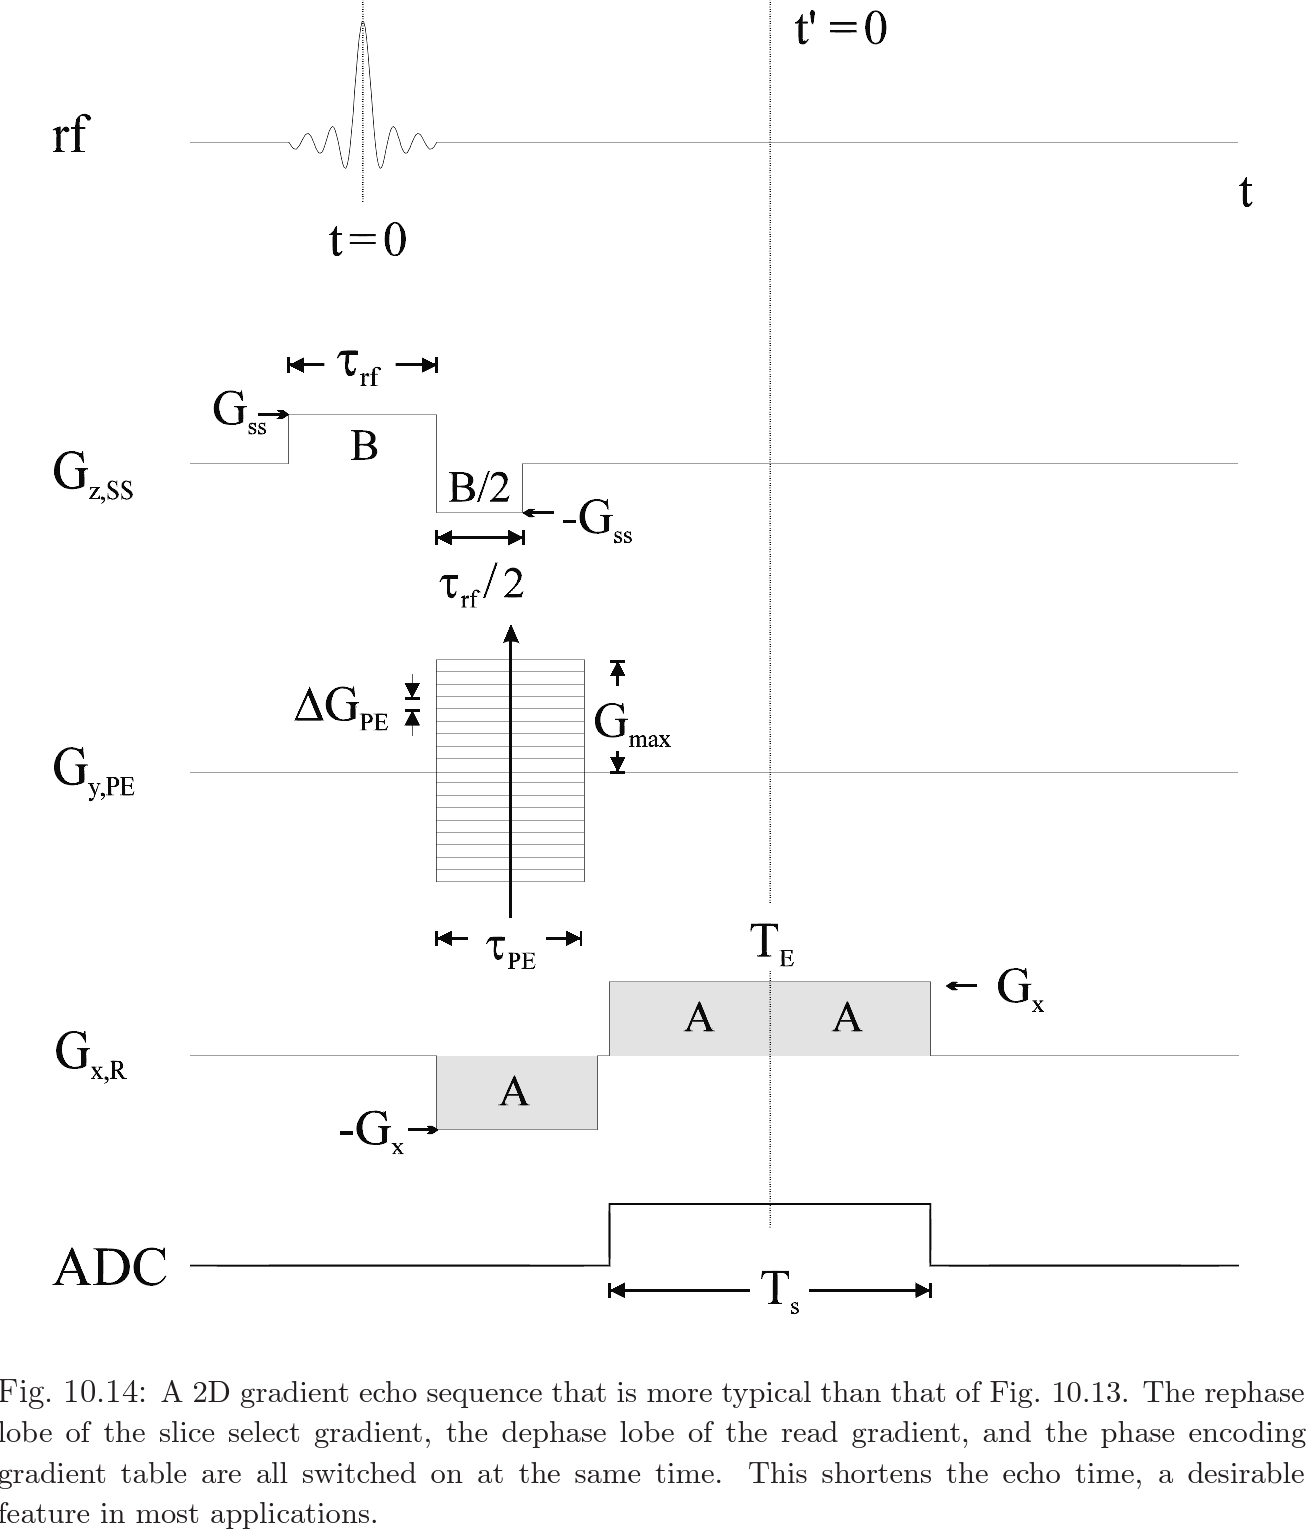
\includegraphics[trim={0cm 0cm 0 0},clip, keepaspectratio,width=0.99\textwidth]{sliceselection}\label{fig:sliceselection}\end{figure}
\end{column}
\begin{column}{0.45\textwidth}
Slice selection, $f(z)=f_0+\gammabar G_zz$: $z_0\pm\frac{\Delta z}{2}$ quindi $f_{RF}=\gammabar G_zz_0-\gammabar G_z\frac{\Delta z}{2}\gammabar G_zz_0+\gammabar G_z\frac{\Delta z}{2}$, cio\'e $BW_{RF}=\Delta f$. Imponiamo che nella slice il flip-angle sia uniforme.
\begin{align*}
&RF(f)=\rect{\frac{\Delta f}{f}}:\\
&-\gammabar G_z\frac{\Delta z}{2}\leq f\leq \gammabar G_z\frac{\Delta z}{2}\\
&B_1(t)=\sinc{(\pi\Delta f t)}
\end{align*}
Rephasing gradient: $\frac{|\int d tG_{rephase}|}{|\int d tG_{SS}|}=50\%$.
\end{column}
\end{columns}
\end{frame}

\begin{wordonframe}{2D slice selection parameters}
\begin{figure}[!ht]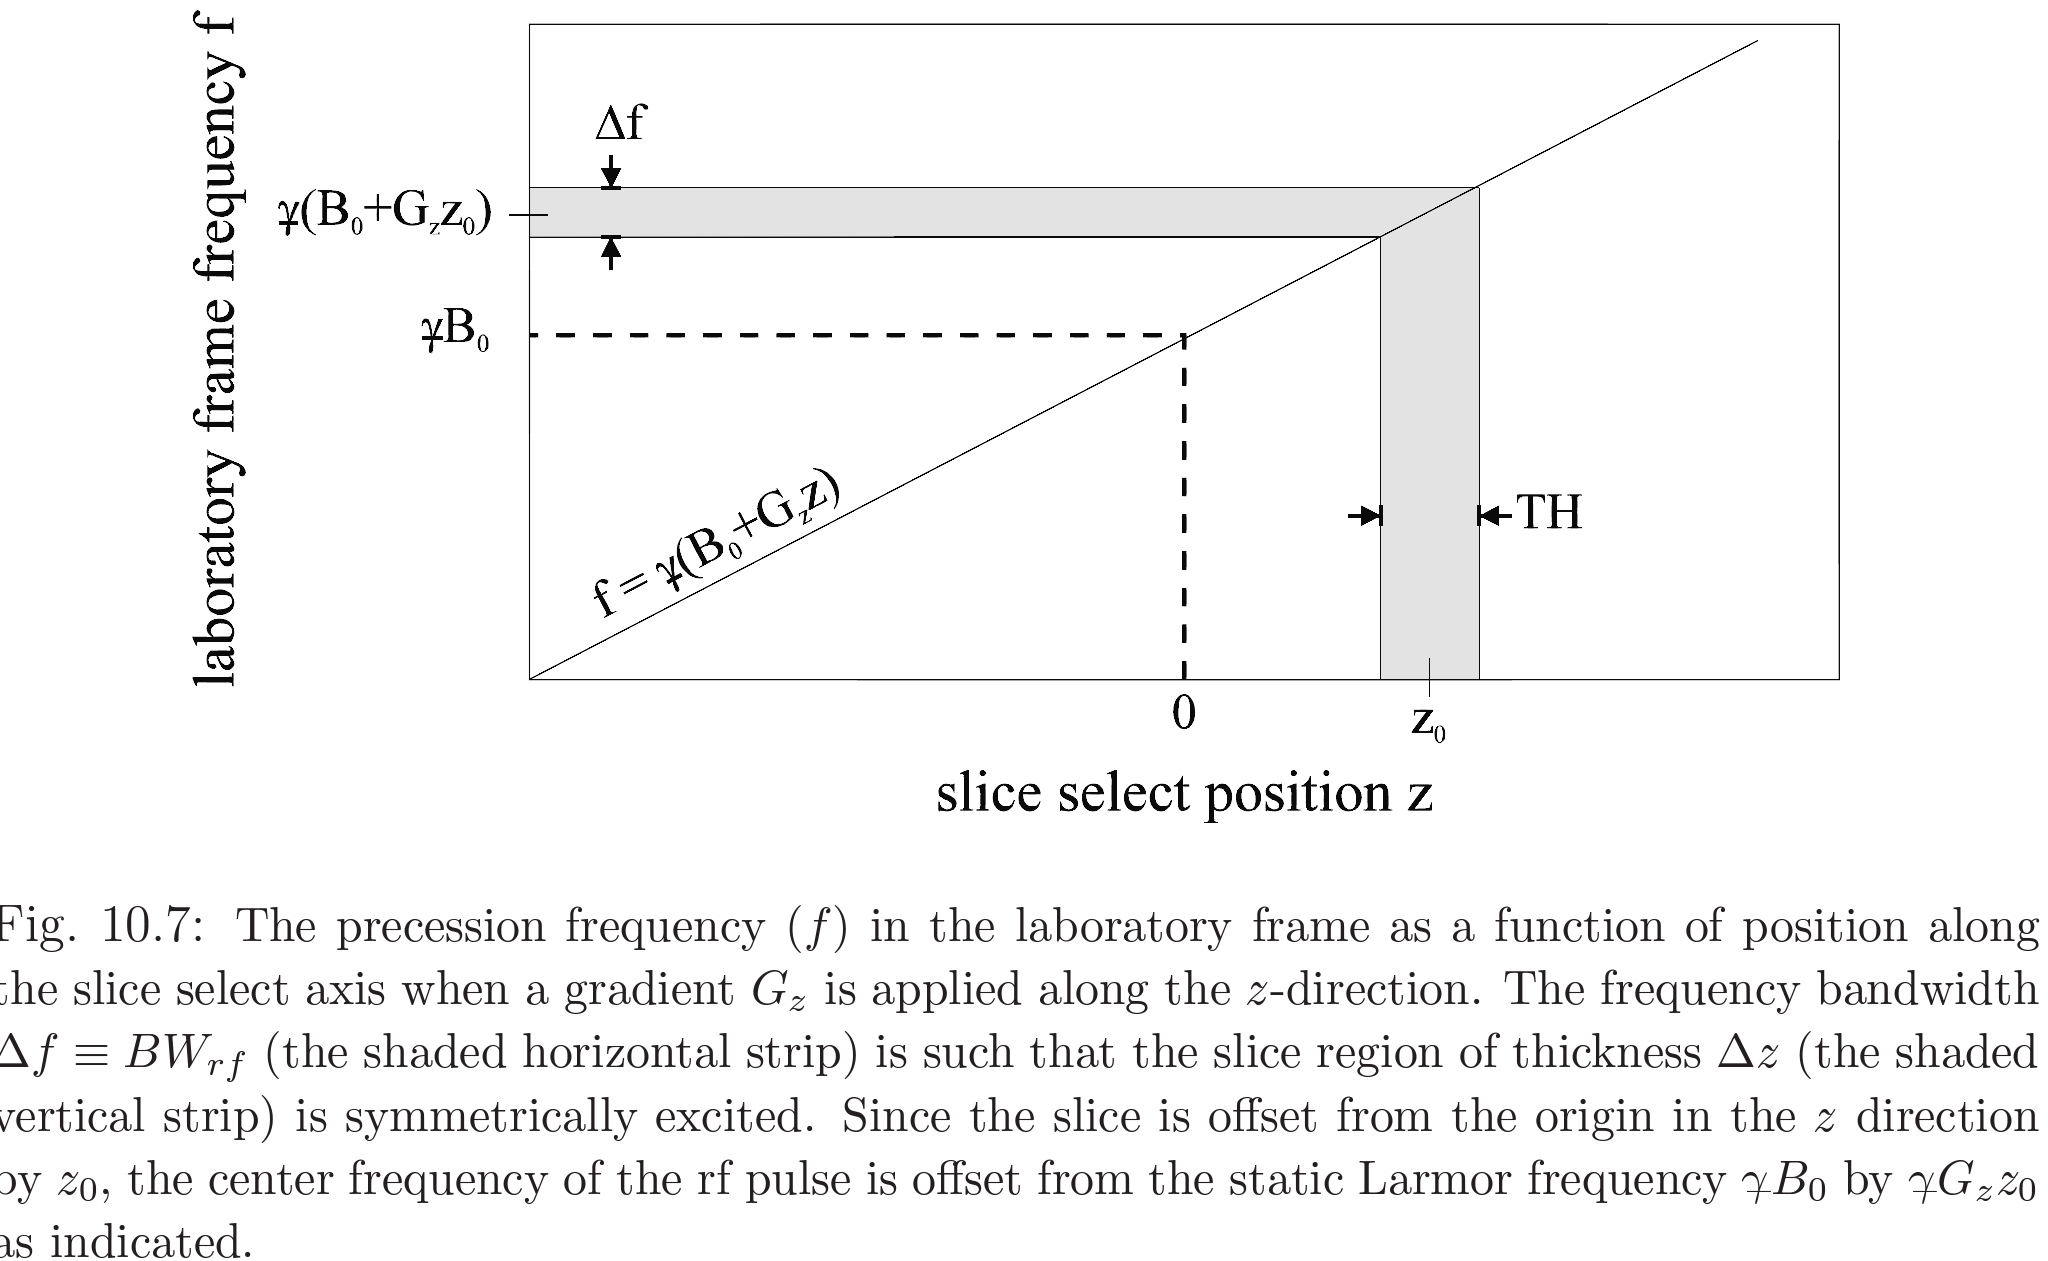
\includegraphics[trim={0cm 0cm 0 0},clip, keepaspectratio,width=0.99\textwidth]{sliceGBW}\label{fig:sliceGBW}\end{figure}
\end{wordonframe}

\section{Filtering and resolution in Fourier T imaging}

\begin{frame}{Nyquist criterion and resolution}
$\frac{1}{\Delta k}=L=FOV$, A object size:
\begin{align*}
&\Delta k<\frac{1}{A}\\
&(\Delta k_R=\gammabar\int_t^{t+\Delta t}d t'G_R(t')=\frac{1}{L_R}<\frac{1}{A_R})\\
&f_R=BW_{read}=\frac{1}{\Delta t}=\gammabar G_RL_R>\gammabar G_RA_R
\end{align*}
Risoluzione: $\Delta x=\frac{1}{2n\Delta k}$, $k=(-n\Delta k,(n-1)\Delta k)$.
\end{frame}

\begin{frame}{FOV and spatial resolution}
    \begin{block}{Limited F imaging: partial k-space coverage}
    Time limitation restrict data sampled per readout ($N_x$), phase encoding ($N_y$) and partition encoding ($N_z$): reconstructed spin data for finite sampling $\hat{\rho}$.
    \begin{equation*}
        \rho(x)=\Delta k\sum_{p=-n}^{n-1}s(p\Delta k)\exp{i2\pi p\Delta k_x}
    \end{equation*}
    $W=2n\Delta k=$
    \end{block}
    \begin{block}{Aliasing (Nyquist criterion) and spatial resolution}
    To avoid aliasing $L=\FOV{}>A$: field of view $L=\invers{\Delta k}$ greater than object dimension.
    \end{block}
\begin{block}{Spatial resolution}
L'altra meta della trasformata di Fourier discreta
\begin{equation*}
s(k)=\Delta x\sum_{q=-n}^{n-1}\rho(q\Delta x)\exp{-i2\pi kq\Delta x}
\end{equation*}
Spatial resolution: $\Delta x=\frac{L}{N}=\frac{1}{N\Delta k}=\frac{1}{W}$ con $N=2n$.
\end{block}
\end{frame}

\begin{frame}{Filter and PSF}
A k-space filter $H(k)$ is a function that multiplies k-space MRI data, the F trasform is the associated PDF $h(x)$: $\rho(x)\to h(x)\circledast \rho(x)$.
\begin{block}{Continuus sampled truncated data}
\begin{align*}
&H_w(k)=\rect{(\frac{k+\Delta k/2}{W})}\\
&s_w(k)=s(k)H_w(k)
\end{align*}
\end{block}
\begin{block}{Gibbs ringing}
Fourier series repr. of function with steps
\end{block}
\begin{block}{Spatial resolution filter}
For arb. imaging method with PSF $h_{filter}(x)$ the spatial resolution is the area under the filter divide by $h(0)$:
\begin{equation*}
\Delta x_{filter}=\text{filter's blur}=\frac{1}{h_f(0)}\int d\,xh_f(x)=\frac{H_f(0)}{h_f(0)}
\end{equation*}
\end{block}
\end{frame}

\begin{frame}{$T_2^*$ decay effects}
When sampling time $T_s=\frac{2n\Delta k}{\gammabar|G|}$ is comparable to $T_2^*$ the exponential decay has filtering action on $s(k)$: filter model $\exp{-t'/T_2^*}$
\begin{equation*}
H_f(k)=\exp{-|k|/(\gammabar GT_2^*)}
\end{equation*}
approximable in most MRI cases ($\Delta k=\gammabar|G|\Delta t\ll\gammabar|G|T_2^*$):
\begin{equation*}
\Delta x_{T_2^*f}=\Delta x\frac{\alpha}{1-\exp{-\alpha}}
\end{equation*}
with $\alpha=\frac{T_s}{2T_2^*}$
\end{frame}

\section{Noise and contrast}

\begin{frame}[allowframebreaks]{Signal and thermal noise}
\begin{block}{Segnale misurato}
Segnale misurato $s_m(k)$ somma $s_m(k)=s(k)+\epsilon(k)$ con funzione di autocorrelazione del rumor
\begin{equation*}
    R_{\epsilon}(\tau)=\exv{\epsilon(k_p)\epsilon^*{k_q}}|_{\tau=k_p-k_q}=\sigma_m^2\delta(\tau)
\end{equation*}
Rumore bianco distribuito normalmente con media 0 e varianza $\sigma_m^2$
\end{block}
\begin{block}{Noise in image domain}
\begin{align*}
&\eta(p\Delta x)=\frac{1}{N}\sum_{p'}\epsilon(p'\Delta k)\exp{i2\pi p'\Delta kp\Delta x}\\
&\var{(\eta(p\Delta x))}=\sigma_0^2(p\Delta x)=\frac{\sigma_m^2}{N}\\
&\rho_m(p\Delta x)=\rho_{m,0}(p\Delta x)+\eta(p\Delta x)\\
&\sigma_0^2(p\Delta x)|_{3D}=\frac{\sigma_m^2}{N_xN_yN_z}
\end{align*}
\end{block}
\end{frame}

\begin{frame}[allowframebreaks]{SNR and imaging parameters}
\begin{block}{Signal to Noise ratio and multi measures average}
k-space averaged sample
\begin{align*}
&s_{m,av}(k)=\frac{1}{N_{acq}}\sum_{i=1}^{N_a}s_{m,i}(k)\\
&\exv{s_{m,av}(k)}=s(k),\ \sigma_{m,av}(k)=\frac{\sigma_m(k)}{\sqrt{N_{acq}}}
\end{align*}
$\SNR{}$ of k-space signal and of given VXL:
\begin{align*}
&\SNR{(k)}=\frac{\exv{s_{m,av}(k)}}{\sigma_{m,av}(k)}=\sqrt{N_{acq}}\frac{s(k)}{\sigma_m(k)}\\
&\SNR{}/\VXL{}(p\Delta x, q\Delta y, r\Delta z)\propto\frac{\sqrt{N_{acq}}}{\sigma_0}
\end{align*}
\end{block}
\begin{block}{SNR and imaging parameters}
\begin{align*}
&\SNR{}/\VXL{}\propto\frac{\Delta x\Delta y\Delta z\sqrt{N_{acq}}}{\sqrt{\frac{\BWr{}}{N_xN_yN_z}}}\\
&\propto\Delta x\Delta y\Delta z\sqrt{N_{acq}N_xN_yN_z\Delta t}\\
&\Delta t= \frac{1}{\BW_{read}}=\frac{1}{L_x\gammabar G_x},\ T_s=N_x\Delta t\\
&\propto\Delta x\Delta y\Delta z\sqrt{N_{acq}N_xN_yN_zT_s}
\end{align*}
Degrading resolution to improve SNR.
\end{block}
\end{frame}

\begin{frame}{Contrasto}
    \begin{block}{Contrasto tessuto A/B: weighting}
\begin{align*}
&C_{AB}=S_A-S_B\\
&=\rho_{0A}(1-\exp{-\frac{T_R}{T_{1A}}})\exp{-\frac{T_E}{T*_{2A}}}-\rho_{0B}(1-\exp{-\frac{T_R}{T_{1B}}})\exp{-\frac{T_E}{T*_{2B}}}
\end{align*}
Spin density weighting:
\begin{equation*}
\left\{\begin{pmatrix}T_E\ll T_{2A,B}^*\\ T_R\gg T_{1A,B}\end{pmatrix}\right.\Rightarrow C_{AB}\approx\rho_{0A}-\rho_{0B}
\end{equation*}
$T_1$-weighting: $T_E\ll {T_2^*}_{AB}$.
$T_2^*$-weighting: $T_R\gg {T_1}_{AB}$.
\end{block}
Contrast2Noise ratio $\CNR{}$: $CNR_{AB}=\frac{C_{AB}}{\sigma_0}=\SNR{}_A-\SNR{}_B$.
\end{frame}

\section{FAt-Water separation}

\begin{frame}{Fat-Water separation methods}
\begin{columns}
\begin{column}{0.5\textwidth}
\begin{itemize}
    \item Chemical shift. $\Delta f_{fw}=f_f-f_w=-\sigma_{fw}\gammabar B_0$, $\sigma_{fw}\approx3.35\ppm$ (\SI{214}{\hertz} at \SI{1.5}{\tesla})
    \item Selective excitation. Si eccita fat con narrow band impulse then water: water \'e off-resonance by chem shift.
    \item Tissue Nulling. Inversion recovery con $T_I$ short e $T_R$ long ().
    \item Multiple point: acquisendo immagini a $T_E$ diversi si possono separare W/F; $\rho_m(T_E)=\rho_{m,w}+\rho_{m,f}\exp{-i\Delta\omega_{fw}T_E}$.
\end{itemize}
\end{column}
\begin{column}{0.5\textwidth}
\begin{itemize}
    \item $T_{1w}>T_{1f}$: for dhort $T_R$ Water/fat image is reduce by $\frac{s_w}{s_f}\approx\frac{T_R}{T_{1w}}/(\frac{T_R}{T_{1f}})=\frac{T_{1f}}{T_{1w}}$
\end{itemize}
\end{column}
\end{columns}
\end{frame}

\section{Random walks, relaxation and diffusion}

\begin{frame}{Molecular model for $T_2$}
Rapide fluttuazioni nel campo magnetico locale (pi\'u rapide di $\tau_L$): moto browniano, spin.
i-esimo spin \'e lungo $y'$: rapide fluttuazioni nel momento torcente determinano random walk di $\vec{\mu}_i$ sulla sfera unitaria. Distribuzione della fase gaussiana
\begin{equation*}
P(\phi)=\frac{\exp{-\phi^2/(2\exv{\phi_i^2})}}{\sqrt{2\pi\exv{\phi_i^2}}}    
\end{equation*}
e la componente trasversale $M_+$
\begin{equation*}
M_+=\frac{M_0}{\sqrt{2\pi\exv{\phi_i^2}}}\int d\,\phi\exp{i\phi}\exp{-\phi_i^2/(2\exv{\phi_i^2})}=M_0\exp{-\exv{\phi_i^2}/2}
\end{equation*}
\begin{block}{Brownian motion and $T_2$ signal loss}
Precession frequency of spin i around z is $\gamma B_{i,z}$: spin motion every $\tau_2$ and intrinsic B at j position
\begin{align*}
&\phi_i(N\tau_2)=\sum_j\gamma B_{i,z,j}\tau_2,\quad \exv{\phi_i^2(N\tau_2)}=\gamma^2\tau_2^2\sum_j\exv{B_{izj}^2}\to\frac{1}{3}\gamma^2\tau_2^2N\exv{B^2}\\
&M_+=M_0\exp{-\gamma^2\tau_2\exv{B^2}t/6},\quad T_2=\frac{6}{\gamma^2\tau_2\exv{B^2}}
\end{align*}
\end{block}
\end{frame}

\begin{frame}{Diffusion}
$x\to x+\epsilon_i\delta$ every $\tau_d$ seconds
\begin{align*}
&B(j\tau_d)=B(0)+G\delta\sum_i^j\epsilon_i\\
&\phi=-\sum^N\gamma\tau_d\Delta B(j\tau_d)=-G\delta\gamma\tau_d\sum_j^N\sum_i^j\epsilon_i\\
&M_+=M_0\exp{-\gamma^2 G^2\delta^2 t^3/(6\tau_d)}\to M_0\exp{-t/T_2}\exp{-\gamma^2 G^2Dt^3/3}
\end{align*}
\end{frame}